\section*{1) a)}

Der Erwartungswert für $y$:
\begin{align*}
  \langle y \rangle = \mu_y = a + b\cdot \langle x \rangle = -0.5 + 0.6 \cdot 6 = 3.1
\end{align*}
Die Varianz von $y$:
\begin{align*}
  Var(y) = b^2 \cdot Var(x) = b^2 \cdot \sigma_x^2 = 0.36 \cdot 12.25 = 4.41
\end{align*}
Die Standardabweichung von $y$:
\begin{align*}
  \sigma_y = \sqrt{Var(y)} = 2.1
\end{align*}
Der Korrelationsfaktor $\rho$:
\begin{align*}
  \rho = \frac{\sigma_{x|y}}{\sigma_x\,\sigma_y} = \frac{1}{3.5 \cdot 2.1} = \frac{20}{147} \approx 0.136
\end{align*}
Wie man in der Abbildung \eqref{fig:Gauß} sehen kann ist die Population 1 eine 2D-Normalverteilung.

\begin{figure}[H]
  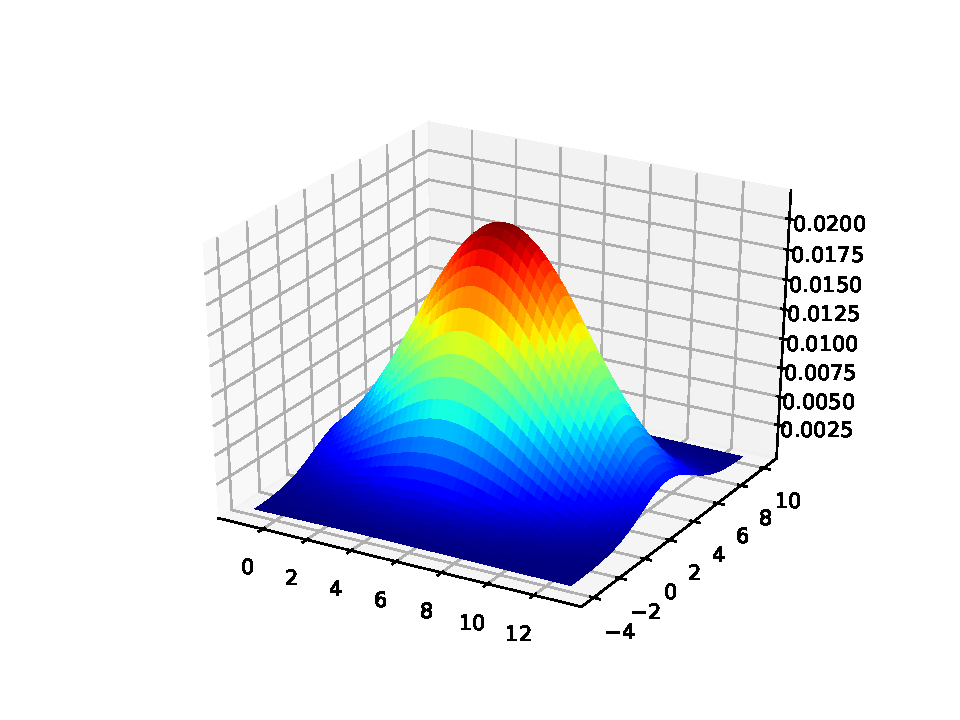
\includegraphics[width=\linewidth]{Python/Aufgabe1a.pdf}
  \caption{Population 1 in einem Plot aufgetragen.}
  \label{fig:Gauß}
\end{figure}


\subsection*{1) b)}
\begin{figure}[H]
  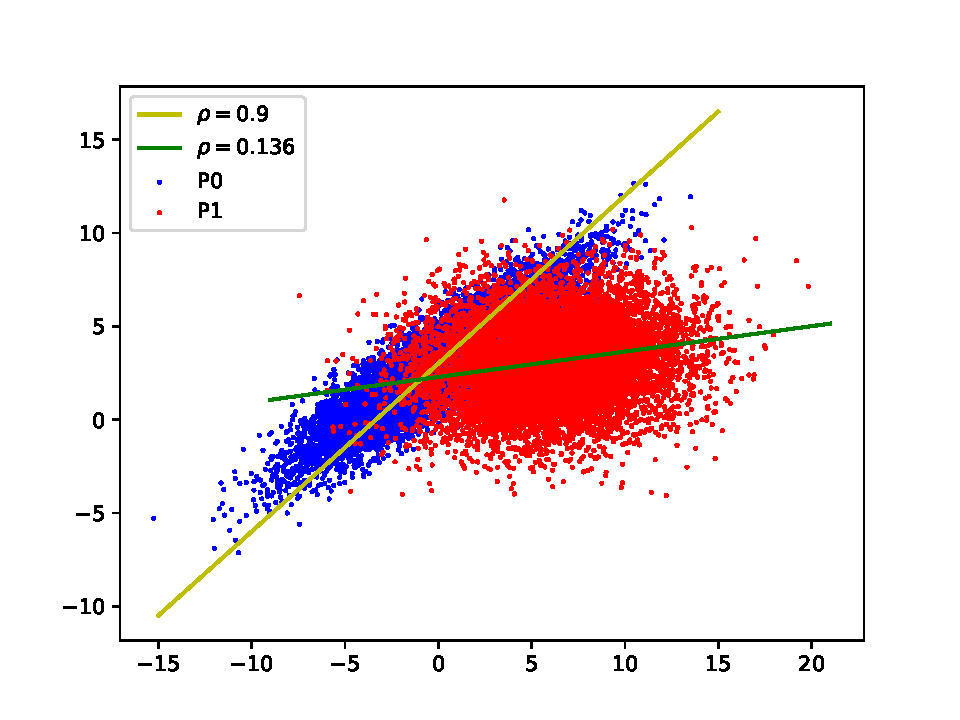
\includegraphics[width=\linewidth]{Python/Aufgabe1b.pdf}
  \caption{Die beiden Populationen in einem Scatter-Plot.}
\end{figure}


\subsection*{1) c)}
Die Zufallszahlen werden von der "numpy.multivariate\_normal"-Funktion erzeugt. Deshalb verändern sich jedes mal die gezogenen Zufallszahlen wodurch sich auch die Stichproben ändern.
\begin{table}[H]
  \centering
  \begin{tabular}{c c c}
    & Stichprobe & exakter Wert \\
    $\mu_{x0}$ & -0.026052 & 0.0 \\
    $\mu_{y0}$ & 2.968815 & 3.0 \\
    $\mu_{x1}$ & 5.999412 & 6.0 \\
    $\mu_{y1}$ & 3.105914 & 3.1 \\
    Var$_{x0}$ & 12.083473 & 12.25\\
    Var$_{y0}$ & 6.600300 & 6.76 \\
    Cov$_0$ & 8.031816 & 8.19 \\
    Var$_{x1}$ & 12.351492 & 12.25 \\
    Var$_{y1}$ & 4.460433 & 4.41 \\
    Cov$_1$ & 0.918914 & 1.0 \\
    $\rho_0$ & 0.899365 & 0.9 \\
    $\rho_1$ & 0.123802 & 0.136 \\
  \end{tabular}
  \caption{Die Werte für die einzelnen Populationen.}
\end{table}

\begin{table}[H]
  \centering
  \begin{tabular}{c c c}
    & Stichprobe \\
    Var$_x$ & 24.591647 \\
    Var$_y$ & 19.062678 \\
    Cov & 20.517091 \\
    $\rho_0$ & 0.947611 \\
  \end{tabular}
  \caption{Die Werte für die Gesamtheit beider Populationen.}
\end{table}





\subsection*{2)}
In den Plots in Abbildung \ref{fig:sca} sind in der Reihenfolge $g_1$, $g_2$ und $g_3$ zu sehen.
\begin{figure}
  \centering
  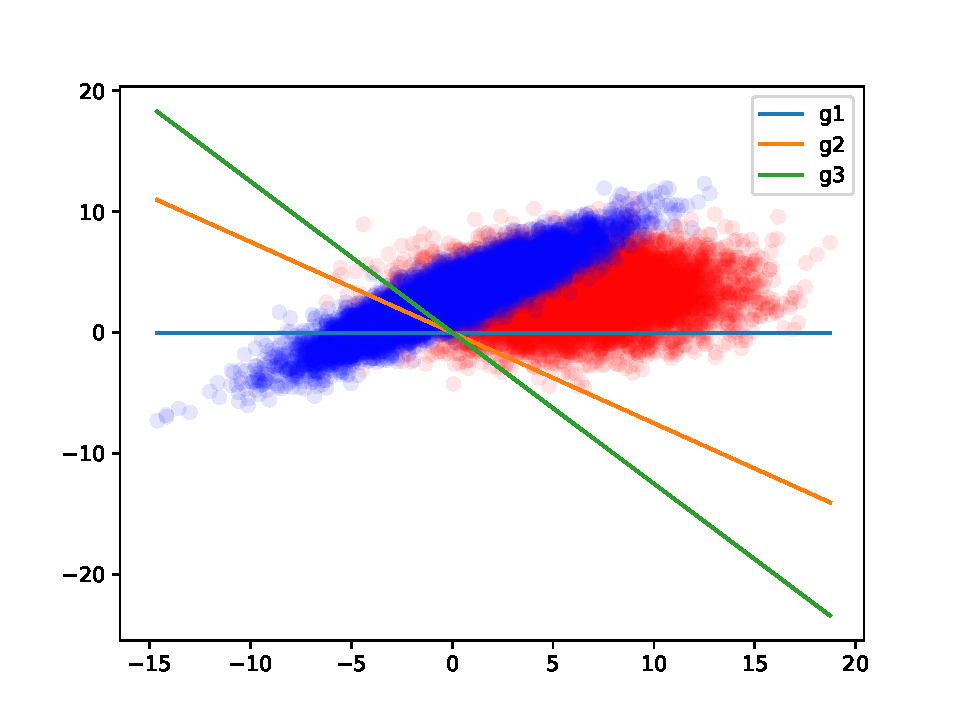
\includegraphics[width=\linewidth]{Python/Scatter.pdf}
  \caption{Scatterplot mit drauf zu Profezierenden Graden}
  \label{fig:sca}
\end{figure}
Im ersten wurden die Messwerte auf die Graden Projeziert und die Populationen in jeweils einen Histogramm dargestellt. Die Projektionsvektoren sind
\begin{eqnarray}
  g1 = \begin{pmatrix}	1 \\ 0 \end{pmatrix}	\\
  g2 = \begin{pmatrix}	-0.6 \\ 0.8 \end{pmatrix} 	\\
  g3 = \begin{pmatrix}	-0.78 \\ 0.62 \end{pmatrix}
\end{eqnarray}
\begin{figure}[H]
  \centering
  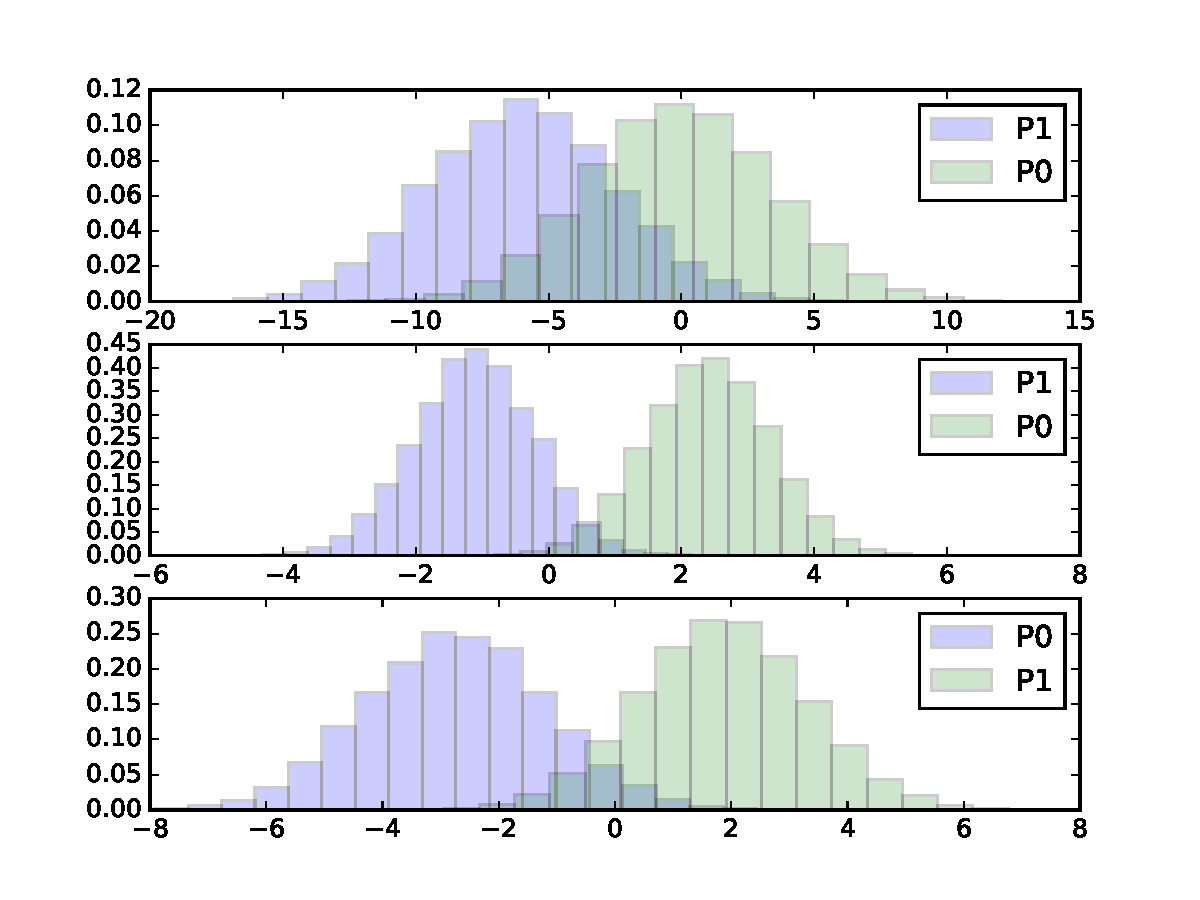
\includegraphics[height=7cm]{Python/hist.pdf}
  \caption{Histogramme der unterschiedlichen Schnitte}
  \label{fig:d}
\end{figure}
Die Reinheit, sowie die Effizienz sind in Abbildung \ref{fig:eff} in Abhängigkeit des Schnittes zu sehen.
\begin{figure}[H]
  \centering
  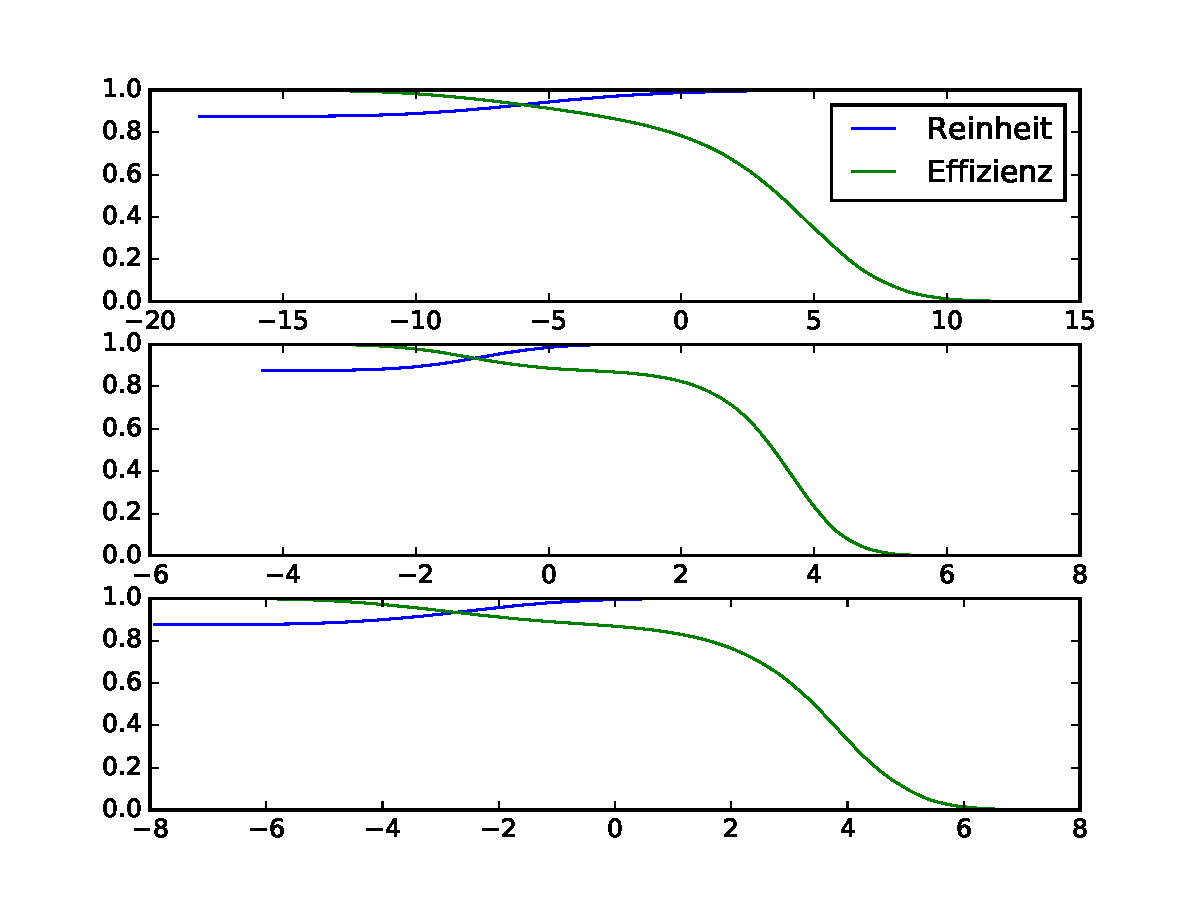
\includegraphics[height=7cm]{Python/cuts.pdf}
  \caption{Reinheit und Effizienz in Abhägigkeit des Ort des Cuts}
  \label{fig:b}
\end{figure}







\subsection*{3) a)}
\begin{align*}
  \mu_0 = \frac{1}{5} \begin{pmatrix} 2 +2 +2 +1 +3 \\ 2 +3 +1 +2 +2 \\ 1 +2 +2 +0 +0 \end{pmatrix} = \begin{pmatrix}2 \\ 2 \\ 1 \end{pmatrix}
\end{align*}
\begin{align*}
  \mu_1 = \frac{1}{5} \begin{pmatrix} 2.5 +2.5 +4 +5.5 +5.5 \\ 2.5 +1.5 +2 +2.5 +1.5 \\ 0 \end{pmatrix} = \begin{pmatrix} 4 \\ 2 \\ 0 \end{pmatrix}
\end{align*}

$S_W = S_0 + S_1$
\begin{align*}
  S_0 &= \begin{pmatrix} 0\\ 0\\ 0\end{pmatrix} \begin{pmatrix} 0& 0& 0\end{pmatrix} + \begin{pmatrix} 0\\ 1\\ 1\end{pmatrix} \begin{pmatrix} 0& 1& 1\end{pmatrix} + \begin{pmatrix} 0\\ -1\\ 1\end{pmatrix} \begin{pmatrix} 0& -1& 1\end{pmatrix} + \begin{pmatrix} -1\\ 0\\ -1\end{pmatrix} \begin{pmatrix} -1& 0& -1\end{pmatrix} \\
  &+ \begin{pmatrix} 1\\ 0\\ -1\end{pmatrix} \begin{pmatrix} 1& 0& -1\end{pmatrix} = \begin{pmatrix} 2&0&0\\ 0&2&0\\ 0&0&4\end{pmatrix} \\
  S_1 &= \begin{pmatrix} -1.5\\ 0.5\\ 0\end{pmatrix} \begin{pmatrix} -1.5& 0.5& 0\end{pmatrix} + \begin{pmatrix} -1.5\\ -0.5\\ 0\end{pmatrix} \begin{pmatrix} -1.5& -0.5& 0\end{pmatrix} + \begin{pmatrix} 0\\ 0\\ 0\end{pmatrix} \begin{pmatrix} 0& 0& 0\end{pmatrix} + \begin{pmatrix} 1.5\\ 0.5\\ 0\end{pmatrix} \begin{pmatrix} 1.5& 0.5& 0\end{pmatrix} \\
  &+ \begin{pmatrix} 1.5\\ -0.5\\ 0\end{pmatrix} \begin{pmatrix} 1.5& -0.5& 0\end{pmatrix} = \begin{pmatrix} 9&0&0\\ 0&1&0\\ 0&0&0\end{pmatrix} \\
  S_W &= \begin{pmatrix} 11&0&0\\ 0&3&0\\ 0&0&4\end{pmatrix}
\end{align*}
\begin{align*}
  S_B = \begin{pmatrix} -2\\ 0\\ 1\end{pmatrix} \begin{pmatrix} -2& 0& 1\end{pmatrix} = \begin{pmatrix} 4&0&-2\\ 0&0&0\\ -2&0&1\end{pmatrix}
\end{align*}



\subsection*{3) b)}
\begin{align*}
  S_W^{-1}\,S_B = \begin{pmatrix} \frac{1}{11}&0&0\\ 0&\frac{1}{3}&0\\ 0&0&\frac{1}{4}\end{pmatrix} \begin{pmatrix} 4&0&-2\\ 0&0&0\\ -2&0&1\end{pmatrix} = \begin{pmatrix} \frac{4}{11}&0&\frac{-2}{11}\\ 0&0&0\\ \frac{-1}{2}&0&\frac{1}{4}\end{pmatrix}
\end{align*}
Berechnung der Eigenwerte $\lambda_i$:
\begin{align*}
  &\det\left(\begin{pmatrix} \frac{4}{11}-\lambda&0&\frac{-2}{11}\\ 0&-\lambda&0\\ \frac{-1}{2}&0&\frac{1}{4}-\lambda\end{pmatrix} \right) = -\lambda\left(\frac{4}{11}-\lambda\right) \left(\frac{1}{4}-\lambda\right) + \frac{\lambda}{11} = -\lambda^3 + \frac{27}{44}\lambda^2 \\
  &\lambda_1 = 0\ , \ \ \ \lambda_2 = \frac{27}{44}
\end{align*}
Berechnung der Eigenvektoren $\vec{r_i}$:
\begin{align*}
  \begin{pmatrix} \frac{4}{11}-\lambda_i&0&\frac{-2}{11}\\ 0&-\lambda_i&0\\ \frac{-1}{4}&0&\frac{1}{4}-\lambda_i\end{pmatrix} \underbrace{\begin{pmatrix} x\\ y\\ z\end{pmatrix}}_{=\vec{r_i}} = \begin{pmatrix} 0\\ 0\\ 0\end{pmatrix}
\end{align*}
$\lambda_1 = 0$
\begin{align*}
  \begin{pmatrix} \frac{4}{11}&0&\frac{-2}{11}\\ 0&0&0\\ \frac{-1}{2}&0&\frac{1}{4}\end{pmatrix} \begin{pmatrix} x\\ y\\ z\end{pmatrix} &= \begin{pmatrix} 0\\ 0\\ 0\end{pmatrix} \\
  \frac{4}{11}x - \frac{2}{11}z &= 0 \\
  0 &= 0 \\
  -\frac{1}{2}x + \frac{1}{4}z &= 0 \\
  \vec{r_1} = \frac{1}{\sqrt{6}} \begin{pmatrix} 1\\ 1\\ 2\end{pmatrix}
\end{align*}

$\lambda_2 = \frac{11}{15}$
\begin{align*}
  \begin{pmatrix} \frac{4}{11}-\frac{27}{44}&0&\frac{-2}{11}\\ 0&-\frac{27}{44}&0\\ \frac{-1}{2}&0&\frac{1}{4}-\frac{27}{44}\end{pmatrix} \begin{pmatrix} x\\ y\\ z\end{pmatrix} &= \begin{pmatrix} 0\\ 0\\ 0\end{pmatrix} \\
  -\frac{1}{4}x - \frac{2}{11}z &= 0 \\
  \frac{27}{44}y &= 0 \\
  -\frac{1}{2}x - \frac{4}{11} z &= 0 \\
  \vec{r_2} = \frac{2}{\sqrt{185}} \begin{pmatrix} 4\\ 0\\ -\frac{11}{2} \end{pmatrix}
\end{align*}



\subsection*{3) c)}
\begin{align*}
  \vec{\lambda} = S_W^{-1}(\vec{\mu_0}-\vec{\mu_1}) = \begin{pmatrix} \frac{1}{11}&0&0\\ 0&\frac{1}{3}&0\\ 0&0&\frac{1}{4}\end{pmatrix} \begin{pmatrix}-2 \\ 0 \\ 1 \end{pmatrix} = \begin{pmatrix} -\frac{2}{11} \\ 0 \\ \frac{1}{4} \end{pmatrix}
\end{align*}



\subsection*{3) d)}
\begin{align*}
  \vec{\lambda}_{norm} = \frac{44}{\sqrt{185}} \begin{pmatrix} -\frac{2}{11} \\ 0 \\ \frac{1}{4} \end{pmatrix} = \frac{1}{\sqrt{185}}  \begin{pmatrix} -8 \\ 0 \\ 11 \end{pmatrix}
\end{align*}
\begin{align*}
  S_{0,proj} &= \frac{1}{\sqrt{185}} \{-5, 6, 6, -8, -24\} \\
  S_{1,proj} &= \frac{1}{\sqrt{185}} \{-12, -12, -32, -44, -44\}
\end{align*}

\begin{figure}[H]
  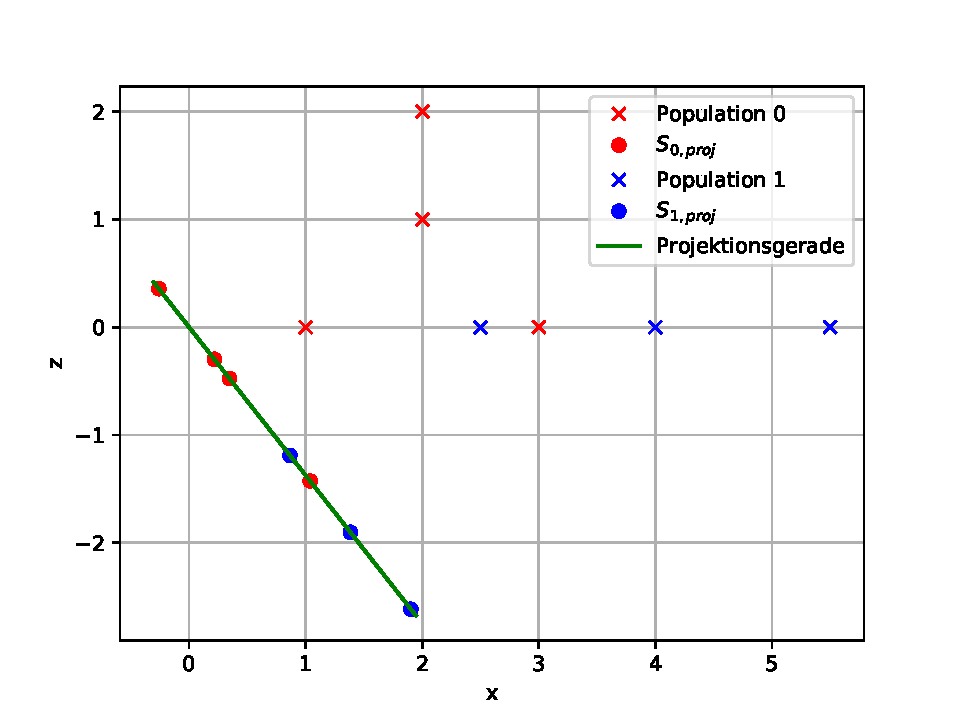
\includegraphics[width=\linewidth]{Python/Aufgabe3d.pdf}
  \caption{Die beiden Populationen auf den Projektionsvektor projiziert.}
\end{figure}




\subsection*{3) e)}
\begin{figure}[H]
  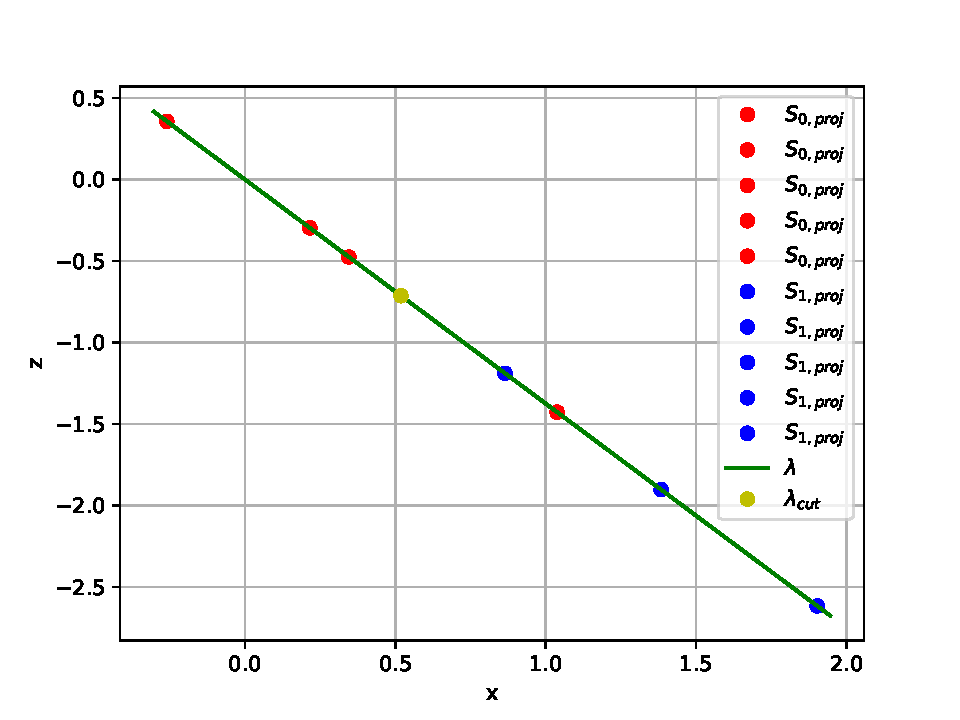
\includegraphics[width=\linewidth]{Python/Aufgabe3e.pdf}
  \caption{Die Projektionsgerade mit den Projizierten Punkten und $\lambda_{cut}$.}
\end{figure}
Wir haben $\lambda_{cut} = -12$ gewählt um eine Reinheit von 1 zu erhalten.
\begin{align*}
  tp = 4, tn = 1, fp = 0, fn = 5 \\
\end{align*}
Wobei $p$ der Population 0 (rot) und $n$ der Population 1 (blau) entspricht. $t$ bedeutet das $p$ und $n$ größer als $\lambda_{cut}$ sind bzw. $f$ das $p$ und $n$ kleiner als $\lambda_{cut}$ sind.
\begin{align*}
  Reinheit = \frac{tp}{tp + fp} = 1 \\
  Effizienz = \frac{tp}{tp + fn} = \frac{4}{9} \approx 0.44 \\
  Genauigkeit = \frac{tp + fn}{tp + tn + fp + fn} = 0.9
\end{align*}




\subsection*{4) a)}
\textbf{Lineare (Fisher) Diskriminanzanalyse:} \\
Die LDA soll zwei Klassen mit $n$ Observablen durch eine (n-1)-dim Hyperebene optimal trennen. Wird zum Beispiel bei der Trennung von einem Rauschen und eines Signal verwendet. Dadurch wird das Signal besser erkennbar bzw. überhaupt erkennbar. \\
\textbf{Feature Extraction:} \\
Die Feature Extraction soll mehrere Attribute zusammenfassen oder transformieren und daraus neue Attribute erstellen. Beipielsweise können ringförmig angeordnete Verteilungen, mit Hilfe von Polarkoordinaten in eine lineare Verteilung transformiert werden. \\
\textbf{Feature Selection:} \\
Die Feature Selection verwirft vorhandene Attribute um ein Subset zu finden. Dafür wird zum Beispiel der "Brute Force"-Algorithmus verwendet, welcher durch einfaches ausprobieren aller Möglichkeiten das beste Ergebnis findet(nicht praktikabel). Die Forward-/Backward-Selection ist ein iteratives Verfahren, welches entweder von vorne oder hinten durch alle Messwerte durchläuft und erst bei einer angegeben Qualität stopt. \\
\\
Außerdem müssen alle missverständlichen Werte, wie NaN oder Inf, durch bessere Werte ersetzt oder entfernt werden. Zusätzlich dazu müssen konstante Attribute oder Attribute mit zu vielen fehlenden Werten entfernt werden.



\subsection*{4) b)}
Eine Normierung ist Sinnvoll. \\
Bei der LDA werden normierte Punkte zum Beispiel orthogonal auf die Hyperebene abgebildet, nicht normierte Punkte werden nicht unbedingt orthogonal abgebildet.



\subsection*{4) c)}
Lücken in den Daten werden durch die Mittelwerte der Verteilung aufgefüllt.



\subsection*{4) d)}
Die Datensätze müssen kombinierbar sein, dafür müssen sie die gleichen Attribute haben und gleich viele Einträge besitzten.
